\documentclass[conference,compsoc]{IEEEtran}
\IEEEoverridecommandlockouts

\usepackage{cite}
\usepackage{ulem}
\usepackage{comment}
\usepackage{amsmath,amssymb,amsfonts}
\usepackage{algorithmic}
\usepackage{graphicx}
\usepackage{textcomp}
\usepackage{enumerate}
\usepackage{enumitem}
\usepackage{xcolor}
\usepackage{soul}
\usepackage{hyperref}
\usepackage[utf8]{inputenc}
\usepackage{multirow}
\def\BibTeX{{\rm B\kern-.05em{\sc i\kern-.025em b}\kern-.08em
    T\kern-.1667em\lower.7ex\hbox{E}\kern-.125emX}}
\newcommand{\mypara}[1]{\smallskip \\ \noindent \textbf{#1: }}


\author{\IEEEauthorblockN{Karen Sowon\IEEEauthorrefmark{1}, Edith Luhanga\IEEEauthorrefmark{2}, Lorrie Faith Cranor\IEEEauthorrefmark{1}, Giulia Fanti\IEEEauthorrefmark{1}, Conrad Tucker\IEEEauthorrefmark{1} and Assane Gueye\IEEEauthorrefmark{2}}
\IEEEauthorblockA{\IEEEauthorrefmark{1}
Carnegie Mellon University}
\IEEEauthorblockA{\IEEEauthorrefmark{2}Carnegie Mellon University-Africa}
}

\begin{document}
\pagenumbering{arabic}


\title{The Role of User-Agent Interactions on\\ Mobile Money Practices in Kenya and Tanzania}
\maketitle

\begin{abstract}
Digital financial services have catalyzed financial inclusion in Africa. Commonly implemented as a mobile wallet service referred to as mobile money (MoMo), the technology provides enormous benefits to its users, some of whom have long been unbanked. While the benefits of mobile money services have largely been documented, the challenges that arise---especially in the interactions between human stakeholders---remain relatively unexplored. In this study, we investigate the practices of mobile money users in their interactions with mobile money agents. We conduct 72 structured interviews in Kenya and Tanzania (n=36 per country). The results show that users and agents design workarounds in response to limitations and challenges that users face within the ecosystem. These include advances or loans from  agents, relying on the user-agent relationships in place of legal identification requirements, and altering the intended transaction execution to improve convenience. Overall, the workarounds modify one or more of what we see as the core components of mobile money: the user, the agent, and the transaction itself.  The workarounds pose new risks and challenges for users and the overall ecosystem. The results suggest a need for rethinking privacy and security of various components of the ecosystem, as well as policy and regulatory controls to safeguard interactions while ensuring the usability of mobile money. 
\end{abstract}

\begin{IEEEkeywords}
Mobile Money, user-agent interaction, digital financial systems, usable privacy and security, technology workarounds
\end{IEEEkeywords}

\section{Introduction}
\label{sec:intro}

\subsection{Motivation}

Reliable estimation of a signal (or image) from nonlinear observations is of fundamental interest to several signal processing and machine learning applications. However, such an estimation is confounded by cases where the nonlinearity in each observation is well-modeled by a \emph{periodic} function such as a sinusoidal function, or sawtooth function, or a square-wave function. Periodic functions are many-to-one mappings, and inverting them can be challenging.

Our focus in this paper is a special kind of periodic nonlinear observation model encountered in high-dynamic range (HDR) imaging. It is well known that real world scenes contain a large range of brightness levels. However, due to hardware limitations, not all brightness levels can be accurately captured using conventional photography; if tuned incorrectly, most scene intensity levels can lie in the saturation region of the image sensors, causing loss of scene information. Similar problems arise in the case of multiplexed imaging systems, such as lensless and coded aperture imaging~\cite{codedaperture,asif2017flatcam}.

%While increasing the dynamic range can solve this problem, it is an impractical strategy since imaging sensors need to have infinite dynamic range, which is infeasible. 
One solution is to increase the dynamic range of the image sensors, but this can lead to expensive hardware. An alternative solution is to deploy a special type of image sensor that {wraps} the observed intensity value at a pixel over a given dynamic range. This is analogous to the familiar \emph{modulo} operation with respect to a parameter $R$, and we call this stylized imaging system a \emph{modulo camera}~\cite{ICCP15_Zhao}.  
Fig.~\ref{fig:func}(a) (black) depicts the modulo nonlinearity, and a major challenge is to undo the effect of this transformation for each observed pixel.

An added challenge in HDR imaging arises due to \emph{quantization}. In fact, the ``true" observations in a modulo camera are quantized versions of the (idealized) modulo observation, and the errors caused in the quantization propagates into the estimation process. Loss of information in the quantization process is unavoidable in principle, and the effect of quantization is magnified with fewer quantization levels. In acquisition systems with low bit-depth, such estimation errors can be very pronounced. Fig.~\ref{fig:func}(a) (cyan) depicts the quantization nonlinearity incurred during the observation process.

\subsection{Setup}

We formalize the above discussion as follows. Assume $\mathcal{X} \subseteq \R^{n}$ to be a given (known) subset in the data space, and consider a signal (or image) $x \in \mathcal{X}$. We model (possible) multiplexing operations and gain adjustments as linear transformations, denoted by $A\in\mathbb{R}^{p\times n}$ and $C\in\R^{m\times p}$ respectively. The composite observation model becomes:
\begin{equation}
\label{quan_obs}
u=f(Ax),~y=Q(Cu),
\end{equation}
where $f(\cdot)=\mod(\cdot,R)$ denotes the modulo function with respect to a range parameter $R$ and $Q(\cdot)$ denotes a quantization function. In this paper, we consider a 1-bit quantization function with only two levels, $0$ and $1$. A representative example is shown in Fig.\ \ref{fig:func} where $A$ and $C$ are identity operators. In  Figs~\ref{fig:func}(c)  and~\ref{fig:func}(d), the outputs of the functions $f$ and $Q$ are displayed when a test grayscale image (Fig.\ \ref{fig:func}(a)) is used in the input. Our overall objective is to estimate the original signal $x$ from the set of measurements $y$. 

%%%%%%%%%%%%%%%%%%%%%%%%%%%%%%%%%%%%%
\begin{figure}[t]
	
	\begin{center}
		\begingroup
		\setlength{\tabcolsep}{0.1pt} % Default value: 6pt
		\renewcommand{\arraystretch}{.1} % Default value: 1
		\begin{tabular}{ccc}      %{c@{\hskip .1pt}c@{\hskip .1pt}c}
			\multicolumn{3}{c}{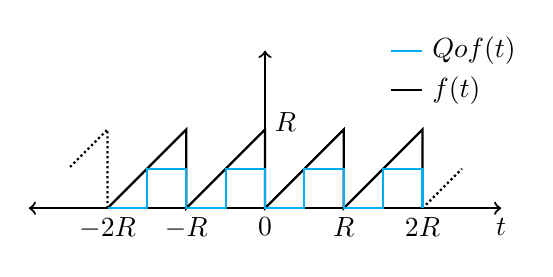
\begin{tikzpicture}
				\draw[<->,thick] (-3,0)--(3,0) node[anchor=north]{$t$};
				\draw (0,0) node[anchor=north]{$0$};
				\draw (0,1.1) node[anchor=west] {$R$};
				\draw (1,0) node[anchor=north]{$R$};
				\draw (2,0) node[anchor=north] {$2R$};
					\draw (-1,0) node[anchor=north]{$-R$};
				\draw (-2,0) node[anchor=north] {$-2R$};
				\draw[] (2,2) node[anchor=west] {{$Qof(t)$}};
				\draw[cyan,thick] (1.6,2) -- (2,2);
				%\draw [densely dotted,thick] (-2.5,1)--(3,1);
				\draw[->,thick] (0,0)--(0,2);
				\draw[] (2,1.5) node[anchor=west] {{$f(t)$}};
				\draw[thick] (1.6,1.5) -- (2,1.5);
				\draw[thick] (-2,0) --(-1,1)-| (-1,0) -- (0,1) -| (0,0) --(1,1)-| (1,0) -- (2,1) -| (2,0);
				\draw[densely dotted,thick] (2,0)--(2.5,0.5);
				\draw[densely dotted,thick] (-2,0)|-(-2,1) -- (-2.5,0.5);
				\draw[thick, cyan] (-2,0) -- ++(0.5,0)-| ++(0,0.5) -- ++(0.5,0) -| ++(0,-0.5) -- ++(0.5,0)-| ++(0,0.5) -- ++(0.5,0) -| ++(0,-0.5) -- ++(0.5,0)-| ++(0,0.5) -- ++(0.5,0) -| ++(0,-0.5) -- ++(0.5,0)-| ++(0,0.5) -- ++(0.5,0) -| ++(0,-0.5);
				\end{tikzpicture}}\\
			\multicolumn{3}{c}{(a)}\\
			\includegraphics[trim = 10mm 60mm 25mm 40mm,clip, width = 0.32\linewidth]{./orgimg.pdf}&
			\includegraphics[trim = 10mm 60mm 25mm 40mm,clip, width = 0.32\linewidth]{./modimg.pdf}&
			\includegraphics[trim = 10mm 60mm 25mm 40mm,clip,width = 0.32\linewidth]{./quantimg.pdf} \\
			(b) & (c) & (d)
		\end{tabular}
		\endgroup
	\end{center}
	\caption{\small{\emph{ (a) Modulo function, $f(t) = \mod(t,R)$ and quantized modulo function, $Qof(t)$; (b,c,d) Depiction of forward model. An input image (b) is transformed via a modulo function $f(t) = \mod(t,R)$, to (c). Such a ``modulo" image is further quantized to obtain (d).}}}
	\label{fig:func}
\end{figure}
%%%%%%%%%%%%%%%%%%%%%%%%%%%%%%%%%%%%%%%%%%%%%%%%%%

\subsection{Our contributions}

Clearly, the above estimation procedure is challenging due to the highly non-invertible nature of the observation model. In this paper, we design a systematic approach that takes some initial steps towards resolving this challenge. Our overarching assumption is that the measurement operations $A$ and $C$ are part of the design space. The core idea in our approach is that a very small, but carefully designed, non-adaptive set of measurements can support efficient estimation of the unknown signal.

Our approach follows stagewise. First, we consider the problem of inverting the quantization function, i.e., recovering $u$ from $y = Q(Cu)$. We demonstrate the existence of a linear operator $C$ (together with an efficient reconstruction algorithm) that supports such an inversion. Specifically, our operator $C$ obeys a particular block-diagonal form with weights chosen according to a harmonic progression; see Section~\ref{sec:Model} for details. We only consider 1-bit quantization functions, but similar ideas can presumably be extended for a higher number of quantization levels. In addition, our method supports the criterion of \emph{consistent reconstruction} as defined in \cite{jacques2011dequantizing}.

Next, we consider the problem of inverting the modulo operation, i.e., recovering $x$ from $u = f(Ax)$.  We propose an algorithm that builds upon the approach proposed in \cite{SoltaniHegde_ICASSP16}. In particular, we show that if the operator $A$ satisfies a certain \emph{factorization} $A = DB$, then $f$ can be stably inverted. To enable efficient inversion, the matrix $D$ must also be block-diagonal with weights chosen either randomly, or according to a geometric progression. In the former case, the reconstruction algorithm is an extension of the approach of~\cite{SoltaniHegde_ICASSP16}, while in the latter case the reconstruction follows the approach of~\cite{ICCP15_Zhao}.

The above two-stage procedure can be easily adapted to the case where we have some prior knowledge of the original signal $x$. This enables our approach to be used in conjunction with compressive imaging architectures. Common priors used in compressive imaging include \emph{sparsity} in some known orthonormal basis~\cite{foucart2013}. Note that our measurements are highly quantized and the total ``bit" complexity of our observations is far smaller than conventional techniques. Therefore, within our framework, one can choose to increase the number of quantizer measurements (rows of $C$) and/or modulo measurements (rows of $D$) in order to achieve better estimation performance.


Fig.~\ref{fig:demo} displays some representative results using our approach. We begin with a standard ``Peppers" image, compute a modulo transformation with three multiplexed measurements per pixel, and further modulate it with a sequence of three harmonic multipliers per measurement before passing it through a 1-bit quantizer. (In words, the overall ``oversampling factor" in our method is $9\times$.) The final binary measurements displayed in Fig.\ \ref{fig:demo}(a) are given as inputs to our reconstruction algorithm. The results from the first and second stages are displayed as images in Fig.\ \ref{fig:demo}(b). As is visually evident, our method is able to successfully reconstruct the image, as displayed in Fig.\ \ref{fig:demo}(c). 


\begin{figure}[t]
	\begin{center}
		\begingroup
		\setlength{\tabcolsep}{1pt} % Default value: 6pt
		\renewcommand{\arraystretch}{.1} % Default value: 1
		{\setlength{\tabcolsep}{1mm}
		\begin{tabular}{ccc|c|c}      %{c@{\hskip .1pt}c@{\hskip .1pt}c}
			\centering
			\includegraphics[trim = 30mm 60mm 40mm 65mm,clip, width = 0.15\linewidth]{./quant11.pdf}&
			\includegraphics[trim = 30mm 60mm 40mm 65mm,clip, width = 0.15\linewidth]{./quant12.pdf}&
			\includegraphics[trim = 30mm 60mm 40mm 65mm,clip, width = 0.15\linewidth]{./quant13.pdf}&
			\includegraphics[trim = 90mm 125mm 90mm 120mm,clip, width = 0.18\linewidth]{./mod11.pdf}&
				\multirow{3}{20mm}{\includegraphics[trim = 90mm 85mm 90mm 120mm,clip, width = \linewidth]{./dms_img.pdf}}\\
			\includegraphics[trim = 30mm 60mm 40mm 65mm,clip, width = 0.15\linewidth]{./quant21.pdf}& 
			\includegraphics[trim = 30mm 60mm 40mm 65mm,clip, width = 0.15\linewidth]{./quant22.pdf}&
			\includegraphics[trim = 30mm 60mm 40mm 65mm,clip, width = 0.15\linewidth]{./quant23.pdf}&
			\includegraphics[trim = 90mm 125mm 90mm 120mm,clip, width = 0.18\linewidth]{./mod21.pdf}&\\
			\includegraphics[trim = 30mm 50mm 40mm 65mm,clip, width = 0.15\linewidth]{./quant31.pdf}& 
			\includegraphics[trim = 30mm 50mm 40mm 65mm,clip, width = 0.15\linewidth]{./quant32.pdf}&
			\includegraphics[trim = 30mm 50mm 40mm 65mm,clip, width = 0.15\linewidth]{./quant33.pdf}& 
			\includegraphics[trim = 90mm 125mm 90mm 120mm,clip, width = 0.18\linewidth]{./mod31.pdf}&\\[1pt]
			\multicolumn{3}{c|}{(a)} &(b)&{\centering(c)}
		\end{tabular}}
		\endgroup
	\end{center}
	\caption{\small{\emph{Illustration of our approach. A given input image is modulated pixel-wise with three pre-chosen weights, passed through a modulo sensor, modulated again pixel-wise with three weights, and quantized to binary images. The resulting observations are shown in (a). The images in (b) and (c) represent the reconstruction of the modulo images, $\widehat{u}$ and the final image, $\widehat{x}$, respectively.}}}
	
	\label{fig:demo}
\end{figure}



\section{Background}
\label{sec:background}

%\SHAN{I think the background section is too long, maybe we can remove the SO3, SE3 parts, only keep SIM3, ellipsoid, SDF}

Rigid body orientation, pose, and similarity are represented using the $\text{SO}(3)$, $\text{SE}(3)$, and $\text{SIM}(3)$ Lie groups, respectively, defined as:
%
\begin{gather}
\label{eq:LieGroups}
\scaleMathLine{\begin{aligned}
\text{SO}(3) &\triangleq \crl{ \bfR \in \bbR^{3 \times 3} \mid \bfR^\top\bfR = \bfI, \det(\bfR) = 1},\\
\text{SE}(3) &\triangleq \crl{ \begin{bmatrix} \bfR & \bft\\\mathbf{0}^\top & 1 \end{bmatrix} \in \bbR^{4 \times 4} \,\bigg\vert\, \bfR \in SO(3), \bft \in \bbR^3}, \\
\text{SIM}(3) &\triangleq \crl{ \begin{bmatrix} s\bfR & \bft\\\mathbf{0}^\top & 1 \end{bmatrix} \in \bbR^{4 \times 4} \,\bigg\vert\, \bfR \in SO(3), \bft \in \bbR^3, s \in \bbR}.
\end{aligned}}
\raisetag{10ex}
\end{gather}
%
We overload $\bfxi_\times$ to denote a mapping from a vector in $\bbR^3$ or $\bbR^6$ or $\bbR^7$ to the Lie algebra $\mathfrak{so}(3)$, $\mathfrak{se}(3)$, or $\mathfrak{sim}(3)$, associated with the Lie groups in \eqref{eq:LieGroups}, defined as:
%
\begin{gather}
\label{eq:LieAlgebras}
\begin{aligned}
\mathfrak{so}(3) &\triangleq \crl{\bfxi_\times = \begin{bmatrix}0 & -\xi_3 & \xi_2\\\xi_3 & 0 & -\xi_1\\-\xi_2 & \xi_1 & 0 \end{bmatrix} \,\bigg\vert\, \bfxi \in \bbR^3},\\
\mathfrak{se}(3) &\triangleq \crl{\bfxi_\times = \begin{bmatrix} \bftheta_\times & \bfrho \\ \mathbf{0}^\top & 0 \end{bmatrix}\,\bigg\vert\, \bfxi = \begin{bmatrix} \bfrho \\ \bftheta\end{bmatrix} \in \bbR^6},\\
\mathfrak{sim}(3) &\triangleq \crl{\bfxi_\times = \begin{bmatrix} \sigma \bfI + \bftheta_\times & \bfrho \\ \mathbf{0}^\top & 0 \end{bmatrix} \,\bigg\vert\, \bfxi = \begin{bmatrix} \bfrho \\ \bftheta \\ \sigma \end{bmatrix} \in \bbR^7}.
\end{aligned}
\raisetag{12ex}
\end{gather}
%
We define an infinitesimal change of a Lie group element $\bfT$ via a left perturbation $\exp\prl{\bfxi_\times}\bfT$, using the exponential map $\exp\prl{\bfxi_\times}$ to retract a Lie algebra element $\bfxi_\times$ to the Lie group. Please refer to \cite[Ch.7]{BarfootBook} or \cite{Gao2017SLAM} for details. 

The coarse shape of a rigid body is represented using a \emph{quadric shape} \cite[Ch.3]{MVGBook}, $\crl{ \bfx \in \bbR^3 \mid \underline{\bfx}^\top \bfQ \underline{\bfx} \leq 0}$, where $\underline{\bfx} \triangleq [\bfx^\top, 1]^\top$ denotes the homogeneous coordinates of $\bfx$ and $\bfQ \in \bbR^{4 \times 4}$ is a symmetric matrix. An axis-aligned ellipsoid centered at the origin:
%
\begin{equation}
\label{eq:ellipsoid}
\mathcal{E}_{\bfu} \triangleq \crl{\bfx \in \bbR^3 \mid \bfx^\top \bfU^{-\top}\bfU^{-1}\bfx \leq 1},
\end{equation}
%
where $\bfU \triangleq \diag(\bfu)$ and the elements of the vector $\bfu \in \bbR^3$ specify the lengths of the semi-axes of $\mathcal{E}_{\bfu}$. An ellipsoid $\mathcal{E}_{\bfu}$ is a special case of a quadric shape with $\bfQ = \diag(\bfU^{-2},-1)$. 
% Instead of as the collection of points $\bfx$ contained in it, 
A quadric shape can also be defined in dual form, as the set of planes $\underline{\boldsymbol{\pi}} = \bfQ\underline{\bfx}$ that are tangent to the shape surface at each $\bfx$. This dual quadric surface definition is $\crl{ \bfpi \in \bbR^3 \mid \underline{\bfpi}^\top \bfQ^* \underline{\bfpi} = 0}$, where $\bfQ^* = \adj(\bfQ)$ is the adjugate of $\bfQ$.
%\footnote{If $\bfQ$ is invertible, $\bfQ^* = \adj(\bfQ) \triangleq \det(\bfQ)\bfQ^{-1}$ can be simplified to $\bfQ^* = \bfQ^{-1} = \diag(\bfU^2, -1)$ due to the scale-invariance of the dual quadric definition.}.
A dual quadric defined by $\bfQ^*$ can be scaled, rotated, or translated by a similarity transform $\bfT \in \text{SIM}(3)$ as $\bfT \bfQ^* \bfT^\top$. Similarity, a dual quadric can be projected to a lower-dimensional space by a projection matrix $\bfP = \begin{bmatrix} \bfI & \mathbf{0} \end{bmatrix}$ as $\bfP \bfQ^* \bfP^\top$.

The fine shape of a rigid body is represented as $\crl{\bfx \in \bbR^3 \mid f(\bfx) \leq 0}$ using the \emph{signed distance field} of a set $\calS \subset \bbR^3$:
%
\begin{equation}
f(\bfx) = \begin{cases}
  -d(\bfx,\partial\calS), & \bfx \in \calS,\\
  \phantom{-}d(\bfx,\partial\calS), & \bfx \notin \calS,
\end{cases}
\end{equation}
%
where $d(\bfx,\partial\calS)$ denotes the Euclidean distance from a point $\bfx \in \bbR^3$ to the boundary $\partial\calS$ of $\calS$.























%% \subsection{SE3}

%This section introduces the necessary mathmatical background. 
%The transformation in $\text{SE}(3)$ can be expressed as:
%\begin{equation}
%\bfT \triangleq \begin{bmatrix} \bfR & \bft\\\mathbf{0}^\top & 1 \end{bmatrix} \in \text{SE}(3)
%\end{equation}
%We overload $\bftheta_\times$ to denote the mapping from an axis-angle vector $\bftheta \in \mathbb{R}^3$ to a $3 \times 3$ skew-symmetric matrix $\bftheta_\times \in \mathfrak{so}(3)$ and the mapping from a position-rotation vector $\bfxi \in \mathbb{R}^6$ to a $4 \times 4$ twist matrix $\bfxi_\times \in \mathfrak{se}(3)$. We define an infinitesimal change of pose $\bfT \in SE(3)$ using a left perturbation $\exp\prl{\bfxi_\times}\bfT \in \text{SE}(3)$ (see~\cite[Ch.7]{BarfootBook}).

%% \subsection{SIM(3)}

%We use the space $\text{SIM}(3)$ of similarity transformations to capture scale $s$ in addition to pose: 
%\begin{equation}
%\bfT \triangleq \begin{bmatrix} s\bfR & \bft\\\mathbf{0}^\top & 1 \end{bmatrix} \in \text{SIM}(3).
%\end{equation}
%We also use $\bfxi$ to denote the corresponding Lie algebra $\mathfrak{sim}(3)$, as in \cite{Gao2017SLAM}:
%\begin{equation}
%\label{eq:sim3_to_SIM3}
%\scaleMathLine[0.91]{
%\begin{aligned}
%\mathfrak{sim}(3) \triangleq
%\left\{\bfxi_\times=
%\left[\begin{array}{cc}
%{\sigma \bfI+\bfphi_\times} & {\bfrho} \\
%\mathbf{0}^\top & {0}
%\end{array}\right] \in \mathbb{R}^{4 \times 4} \;\bigg\vert\; \bfxi = \left[\begin{array}{c}
%{\bfrho} \\
%{\bfphi} \\
%{\sigma}
%\end{array}\right] \in \mathbb{R}^{7}\right\}
%\end{aligned}
%}
%\end{equation}
%We define the operator:
%%\NA{what is the operator $\underline{\bfx}^\circledcirc$?}
%%\SHAN{I don't think we will use $\underline{\bfx}^\circledcirc$ anywhere}
%\begin{equation}
%\underline{\bfx}^\odot \triangleq \begin{bmatrix} \bfI_3 & -\bfx_\times & \bfx\\ \mathbf{0}^\top & \mathbf{0}^\top & 0 \end{bmatrix} \in \mathbb{R}^{4 \times 7}
%\end{equation}




%\begin{definition*}
%The \textit{signed distance field} of a set $\calS \subset \mathbb{R}^3$ is
%\begin{equation}
%f(\bfx) = \begin{cases}
%  -d(\bfx,\partial\calS) & \bfx \in \calS\\
%  d(\bfx,\partial\calS) & \bfx \notin \calS
%\end{cases}
%\end{equation}
%where $d(\bfx,\partial\calS)$ is the distance from a point $\bfx \in \mathbb{R}^3$ to the set boundary $\partial\calS$, and we use $d$ as a shorthand notation to denote this distance.
%\end{definition*}


%\begin{definition*}
%\textit{Huber error function} \cite{Huber1964Robust} with parameter $\delta > 0$ is:
%\begin{equation}
%\rho(r) \triangleq 
%\begin{cases}
%\frac{1}{2}r^2 & |r|\leq \delta,\\
%\delta(|r|-\frac{1}{2}\delta) & \text{else}.
%\end{cases}
%\end{equation}
%\end{definition*}
%whose gradient can be computed as 
%\[
%  \frac{\partial \rho(r)}{\partial r}
%  =\left\{\begin{array}{ll}
%    r & |r| \leq \delta \\
%    \text{sign}(r)\delta  & \text{ else}. 
%    \end{array}\right.
%\] 

%An axis-aligned ellipsoid centered at the origin can be described as:
%\begin{equation}
%\mathcal{E}_{\bfu} \triangleq \crl{\bfx \mid \bfx^\top \bfU^{-\top}\bfU^{-1}\bfx \leq 1},
%\end{equation}
%where $\bfU \triangleq \diag(\bfu)$ and the elements of the vector $\bfu = [a,b,c]^{\top}$ are the lengths of the semi-axes of $\mathcal{E}_{\bfu}$. In homogeneous coordinates, $\mathcal{E}_{\bfu}$ can be represented as a quadric surface~\cite[Ch.3]{MVGBook}, $\crl{ \bfx \mid \underline{\bfx}^\top \bfQ_{\bfu} \underline{\bfx} \leq 0}$, where $\bfQ_{\bfu} = \mathbf{diag}(\bfU^{-2},-1)$. This describes the ellipsoid as a collection of points lying on its surface. 

%Alternatively, a quadric can be defined by the set of planes $\underline{\boldsymbol{\pi}} = \bfQ_{\bfu}\underline{\bfx}$ tangent to its surface at $\underline{\bfx}$. This dual quadric surface is defined as $\crl{ \bfpi \mid \underline{\bfpi}^\top \bfQ_{\bfu}^* \underline{\bfpi} = 0}$, where $\bfQ_{\bfu}^* = \mathbf{adj}(\bfQ_{\bfu})$~\footnote{If $\bfQ_{\bfu}$ is invertible, $\bfQ_{\bfu}^* = \mathbf{adj}(\bfQ_{\bfu}) = \det(\bfQ_{\bfu})\bfQ_{\bfu}^{-1}$ can be simplified to $\bfQ_{\bfu}^* = \bfQ_{\bfu}^{-1} = \diag(\bfU^2, -1)$ due to the scale-invariance of the dual quadric definition.}. A dual quadric defined by $\bfQ_{\bfu}^*$ can be transformed by $\bfT \in SE(3)$ to another reference frame as $\bfQ^* = \bfT \bfQ_{\bfu}^* \bfT^\top$, which can be projected to a lower-dimensional space by $\bfP \in \mathbb{R}^{3\times 4}$ as $\bfP \bfQ^* \bfP^\top$. 
%$\bfQ^*$ can be parameterized as:
%\begin{equation}
%\label{eq:ellipsoid}
%\begin{aligned}
%\bfQ^*
%&=
%\mathbf{T} \bfQ_{\bfu}^* \mathbf{T}^{\top}=
%\left[\begin{array}{cc}
%\mathbf{R} & \bft \\
%\mathbf{0}^{\top} & 1
%\end{array}\right]\left[\begin{array}{cc}
%\mathbf{U} \mathbf{U}^{\top} & \mathbf{0} \\
%\mathbf{0} & -1
%\end{array}\right]\left[\begin{array}{ll}
%\mathbf{R}^{\top} & \mathbf{0} \\
%\bft^{\top} & 1
%\end{array}\right] \\ 
%&=
%\begin{pmatrix} 
%\mathbf{R} \mathbf{U} \mathbf{U}^\top \mathbf{R}^\top -  \bft \bft^\top & - \bft \\ -\bft^\top & -1
%\end{pmatrix}
%\end{aligned}
%\end{equation}




\section{Related Work}
\label{Sec:related work}
We discuss two strands of prior work related to this study: adoption and use of MoMo, and privacy and security of digital financial services.  

\subsection{Adoption of mobile money}
Some studies have identified the barriers to the use of MoMo, most of which mirror the top barriers to account ownership at a formal financial institution. These include cost, unreliable mobile networks and power grids, preference for cash, lack of documentation for KYC requirements, and low literacy---including digital literacy skills \cite{awanis2022state} \cite{demirgucc2022global}. These studies also suggest that although perceived trust of MoMo contributes to its use among users, lack of trust is one of the main barriers cited by non-users \cite{akinyemi2020determinants} \cite{awanis2022state}.

Similarly, technology adoption studies (e.g.,\cite{baganzi2017examining},\cite{abdul2019customers}, \cite{okello2020trust}, \cite{noreen2021impact}, \cite{osakwe2022trust})  have investigated the factors that predict uptake and use of MoMo. Most of these studies are  quantitative investigations that aim to establish antecedents to adoption. The findings in these studies unanimously emphasize the importance of trust as a significant predictor of adoption. Osakwe et al., \cite{osakwe2022trust} further explore factors that can increase trust in MoMo and offer four specific  institutional measures that can support initial trust building. One of the factors is perceived reputation of both the MoMo agents and the MoMo provider. While these studies have been useful in elucidating adoption, none of them explore the interactions that arise from trust between the agents and users, either pre-adoption or post-adoption
\cite{benbasat2005trust} \cite{sowon2020trust}. This trust often influences continued use.

Post adoption, users tend to develop technology coping strategies in response to technology challenges. Other researchers have studied this in relation to technologies like mobile apps, mobile health, and tablets \cite{inal2019users} \cite{sowon2022information} \cite{zamani2021accommodating}. In general, these studies show that users can cope with technology by abandoning it (the flight response) or accommodating if (the fight response). The concept of workarounds that we use to describe alternative workflows in this study can be considered a fight response.
  
\subsection{Mobile financial system privacy and security}
The increased uptake of MoMo has been associated with an increase in fraud that takes advantage of security vulnerabilities in MoMo technologies \cite{reaves2017mo}. Some of the fraud cases center on the role of agents. In 2020, Uganda suspended its MoMo transactions on its network after hackers breached the payment system, resulting in a loss of over \$3 million  \cite{kafeero_2020}. The attack was perpetrated by fraudsters who worked in collaboration with MoMo agents. Researchers have also analyzed the security of MoMo in Uganda and identified the potential sources of security risks \cite{ali2020evaluation}. 
While our study touches on the role of fraud in MoMo users' decision-making,  it is only a small component of our study. More broadly, we want to understand how user beliefs and perceptions affect their interactions with agents and the MoMo system at large, whether those perceptions relate to fraud or not.

Similarly, several research studies have explored MoMo privacy issues, reviewing privacy policies and relevant regulations   \cite{bowers2017regulators} \cite{harris2012privacy}. MoMo is a data-rich environment, and prior work has noted various aspects of the transaction process that may raise privacy concerns \cite{makulilo2015privacy}. These include the identification of subscribers through SIM registration, KYC performed by agents, and the multiple roles that agents play that make them data depositors. The interaction between various stakeholders also introduces layers of complexity for privacy and security in MoMo environments \cite{mogaji2022dark}. Other studies have focused on privacy concerns with related services such as mobile loan apps \cite{munyendo2022desperate} and some have explored the role of human intermediaries on access to digital services. For example, in Kenya,  cybercafe owners sometimes performed services for their patrons such as logging in~\cite{munyendoeighty}.  While addressing privacy, these studies do not specifically evaluate the user-agent interaction. 

In the work most closely related to ours, Mogaji and Nguyen \cite{mogaji2022dark} explore the ``dark side" of MoMo interactions between stakeholders in Nigeria. 
Their study touches on user-agent relationships, from which they observe several similar patterns to those in our work, including unofficial fees from agents and third-party data sharing. 
The most important difference between their work and ours is that we study the user-agent relationship in depth from the perspective of users in Kenya and Tanzania, whereas their work considers multiple stakeholders (including users and agents), and focuses mainly on the downsides of MoMo for financially-vulnerable customers in Nigeria.
As a result, their study does not uncover the same breadth or depth of workarounds or practices that we observe, nor does it probe the underlying causes for these workarounds in as much depth, if at all. 
% !TEX root = Guillon2017_arxiv.tex

\subsection{Experimental design and data pre-processing}

The study involved 25 Alzheimer's diseased (AD) patients (13 women) and 25 healthy age-matched control (HC) subjects (18 women).
All participants underwent the Mini-Mental State Examination (MMSE) for global cognition \cite{folstein_mini-mental_1975} and the Free and Cued Selective Reminding Test (FCSRT) for verbal episodic memory \citep{buschke_cued_1984, grober_screening_1988, pillon_explicit_1993}. Specifically, we considered the Total Recall (TR) score - given by the sum of the free and cued recall scores - which has been demonstrated to be highly predictive of AD \citep{sarazin_amnestic_2007}.

Inclusion criteria for all participants were: \textit{i)} age between 50 and 90; \textit{ii)} absence of general evolutive pathology; \textit{iii)} no previous history of psychiatric diseases; \textit{iv) }no contraindication to MRI examination; \textit{v)} French as a mother tongue.
Specific criteria for AD patients were: \textit{i)} clinical diagnosis of Alzheimer's disease;\textit{ ii)} Mini-Mental State Examination (MMSE) score greater or equal to $18$.
Magnetic resonance imaging (MRI) acquisitions were obtained using a 3T system (Siemens Trio, 32-channel system, with a 12-channel head coil). The MRI examination included a 3D T1-weighted volumetric magnetization-prepared rapid-gradient echo (MPRAGE) sequence with 1mm isotropic resolution and the following parameters: repetition time (TR)=2300 ms, echo time (TE)=4.18ms, inversion time (TI)=900 ms, matrix=256x256. This sequence provided a high contrast-to-noise ratio and enabled excellent segmentation of high grey/white matter.

The magnetoencephalography (MEG) experimental protocol consisted in a resting-state with eyes-closed (EC). Subjects seated comfortably in a dimly lit electromagnetically and acoustically shielded room and were asked to relax and fix a central point on the screen.
MEG signals were collected using a whole-head MEG system with $102$ magnetometers and $204$ planar gradiometers (Elekta Neuromag TRIUX MEG system) at a sampling rate of $1\,000$ Hz and on-line low-pass filtered at $330$ Hz.
The ground electrode was located on the right shoulder blade. An electrocardiogram (EKG) Ag/AgCl electrodes was placed on the left abdomen for artifacts correction and a vertical electrooculogram (EOG) was simultaneously recorded.
% Horizontal and vertical eye position as well as pupil diameter were monitored using an eye tracker (EyeLink 1000, SR research) and recorded together with MEG and EKG data. % => Useless since eyes are closed.
Four small coils were attached to the participant in order to monitor head position and to provide co-registration with the anatomical MRI. The physical landmarks (the nasion, the left and right pre-auricular points) were digitized using a Polhemus Fastrak digitizer (Polhemus, Colchester, VT).

We recorded three consecutive epochs of approximately $2$ minutes each. All subjects gave written informed consent for participation in the study, which was approved by the local ethics committee of the Pitie-Salpetriere Hospital. Signal space separation was performed using MaxFilter \citep{taulu_spatiotemporal_2006} to remove external noise. We used in-house software to remove  cardiac and ocular blink artifacts from MEG signals by means of principal component analysis.
We visually inspected the preprocessed MEG signals in order to remove epochs that still presented spurious contamination.
At the end of the process, we obtained a coherent dataset consisting of three clean preprocessed epochs for each subject.

\subsection{Source reconstruction, power spectra and brain connectivity} \label{subsec:brain_connectivity}

We reconstructed the MEG activity on the cortical surface by using a source imaging technique \citep{he_brain_1999,baillet_evaluation_2001}.
We used the FreeSurfer 5.3 software (surfer.nmr.mgh.harvard.edu) to perform skull stripping and segment grey/white matter from the 3D T1-weighted images of each single subject \citep{fischl_whole_2002, fischl_sequence-independent_2004}. Cortical surfaces were then modeled with approximately $20000$ equivalent current dipoles (i.e., the vertices of the cortical meshes).
We used the Brainstorm software \citep{tadel_brainstorm:_2011} to solve the linear inverse problem though the wMNE (weighted Minimum Norm Estimate) algorithm with overlapping spheres \citep{lin_assessing_2006}. Both magnetometer and gradiometer, whose position has been registered on the T1 image using the digitized head points, were used to localize the activity over the cortical surface.
The reconstructed time series were then extracted from $148$ regions of interest (ROIs) defined by the Destrieux atlas \citep{destrieux_automatic_2010-1}.
% We chose this Atlas for its number of ROIs that is computationally-wise adapted for this application and close to the number of MEG sensors, because it is provided by the FreeSurfer software, because it is a cortical-only atlas and because the regions have similar size hence a similar number of vertices on the cortical mesh.

We computed the power spectral density (PSD) of the ROI signals by means of the Welch's method; we chose a $2$ seconds sliding Hanning window, with a $25\%$ overlap. The number of FFT points was set to $500$ for a frequency resolution of $0.5 \Hz$.
% NOTE: Finding reference for spectral coherence is not useful.
We estimated functional connectivity by calculating the spectral coherence between each pair of ROI signals \citep{carter_coherence_1987}. 
%For a given frequency $f$, the spectral coherence for the channels pair $(i,j)$ can be computed as follow:
%\begin{equation}
	%Coh_{ij}(f) = \frac{ \abs{S_{ij}(f)} }{ \sqrt{S_{ii}(f)S_{jj}(f)} }
	%\label{eq:coherence}
%\end{equation}
%where $S_{ij}(f)$ is the cross-spectrum of two time series $x_i(t)$ and $x_j(t)$ of ROI $i$ and $j$ respectively. We used the same FFT parameters as for the PSD.
As a result, we obtained for each subject and epoch, a connectivity matrix of size $148 \times 148$ where the $(i,j)$ entry contains the value of the spectral coherence between the signals of the ROI $i$ and $j$ at a frequency $f$.

We then averaged the connectivity matrices within the following characteristic frequency bands \citep{stam_generalized_2002,babiloni_abnormal_2004}: $\delta$ (2-4 Hz); $\theta$ (4-8 Hz); $\alpha=\alpha_{1}$ (8-10.5 Hz) and $\alpha_{2}$ (10.5-13 Hz); $\beta=\beta_{1}$ (13-20 Hz) and $\beta_{2}$ (20-30 Hz); $\gamma$ (30-45 Hz).
We further averaged the resulting connectivity matrices across epochs to obtain our raw individual brain networks whose nodes were the ROIs ($n = 148$) and links, or edges, were the spectral coherence values.

\subsection{Single-layer network analysis} \label{subsec:singlelayer}

In order to cancel the weakest noisy connections, we thresholded the values in the connectivity matrices and retained the same number of links in each brain network at every frequency band, or layer.
We considered six representative connection density thresholds corresponding to an average node degree $k=\{1, 3, 6, 12, 24, 48\}$. These values cover the density range $[0.007, 0.327]$ which contains the typical density values used in complex brain network analysis \citep{bullmore_complex_2009,rubinov_complex_2010,de_vico_fallani_graph_2014}.
The resulting sparse brain networks, or graphs,  were represented by adjacency matrices $A$, where the $a_{ij}$ entry indicates the presence or absence of a link between nodes $i$ and $j$.

\subsubsection{Participation coefficient} \label{subsec:pc}

Given a network partition, the local participation coefficient ($PC_i$) of a node $i$ measures how evenly it is connected to the different clusters, or modules of the network \citep{guimera_cartography_2005}.
Nodes with high participation coefficients are considered central hubs as they allow for the information exchange among different modules.
The global participation coefficient $PC$ of a network at layer $\lambda$  is then given by the average of the $PC_i$ values:
\begin{equation}
	PC^{[\lambda]} 	= \frac{1}{n} \sum_{i=1}^{N} PC_i^{[\lambda]}
	=  \frac{1}{n} \sum_{i=1}^{N} \Bigg[ 1-\sum_{m=1}^{M^{[\lambda]}} \Bigg( \frac{k_{i,m}^{[\lambda]}}{k_i^{[\lambda]}} \Bigg)^2 \Bigg] \text{,}
	\label{eq:pc}
\end{equation}
where $k_{i,m}^{[\lambda]}$ is the number of weighted links from the node $i$ to the nodes of the module $m$ of the layer $\lambda$. By construction, $PC$ ranges from $0$ to $1$.
Here, the partition of the networks into modules was obtained by maximizing the modularity function as defined by \cite{newman_finding_2006}.

\subsubsection{Flattened networks} \label{subsec:flattening}

We also computed the participation coefficients for brain networks obtained by flattening the frequency layers into a single \textit{overlapping}  or \textit{aggregated} network \citep{battiston_structural_2014}.
In an overlapping network, the weight of an edge $o_{ij}$ corresponds to the number of times that the nodes $i$ and $j$ are connected across layers:
\begin{equation}
	o_{ij} = \sum_{\lambda} a_{ij}^{[\lambda]} \text{,}
	\label{eq:overlapping}
\end{equation}

In an aggregated network, the existence of an edge indicates that nodes $i$ and $j$ are connected in at least one layer:
\begin{equation}
	a_{ij} = \left\{
	\begin{array}{ll}
		1 & \text{if } \exists{\lambda} : a_{ij}^{[\lambda]} \ne 0 \\
		0 & \text{otherwise}                                       \\
	\end{array}
	\right. \text{,}
	\label{eq:aggregated}
\end{equation}

Notice that, by construction, flattened networks do not preserve the original connection density of the single layer networks.

\subsection{Multi-layer network analysis} \label{subsec:multiplex_networks}
% TODO: Add reference for multiplex definition
We adopted a multi-layer network approach to integrate the information from brain networks at different frequency bands, while preserving their original structure.
We built for each subject a multiplex network (Fig. \ref{fig:multiplex}a,b) where different layers correspond to different frequency bands and each node in one layer is virtually connected to all its counterparts in all the other layers.

Without loss of generality, if we consider the standard neurophysiological frequency bands, the resulting supra-adjacency matrix $\mathcal{A}$ is given by the following intra-layer of adjacency matrices on the main diagonal:
\begin{equation}
	\mathcal{A} = \{ A^{[\delta]}, A^{[\theta]}, A^{[\alpha]}, A^{[\beta]}, A^{[\gamma]} \}\text{,}
	\label{eq:supraadjacency}
\end{equation}
where $A^{[\lambda]}$ is adjacency matrix of the frequency layer $\lambda$. By construction, the inter-layer adjacency matrices of multiplexes are intrinsically defined as identity matrices.

\subsubsection{Multi-participation coefficient} \label{subsec:mpc}
We considered the multi-layer version of the local participation coefficient $MPC_i$ to measure how evenly a node $i$ is connected to the different layers of the multiplex \citep{battiston_structural_2014}.
This way, nodes with high multi-participation coefficients are considered central hubs as they would allow for a better information exchange among different layers.
The global multi-participation coefficient is then given by the average of the $MPC_i$ values:

\begin{equation}
	MPC = \frac{1}{n} \sum_{i=1}^{N} MPC_i
	= \frac{1}{n} \sum_{i=1}^{N} \frac{M}{M-1} \Bigg[ 1-\sum_{\lambda} \Bigg( NLP_i^{[\lambda]} \Bigg)^2 \Bigg] \text{,}
	\label{eq:mpc}
\end{equation}
where $NLP_i^{[\lambda]} = k_i^{[\lambda]} / o_i$, stands for \textit{node-degree layer proportion}, which measures the percentage of the total number of links (i.e. in all layers) of node $i$ that are in layer $\lambda$.
By construction, if nodes tend to concentrate their connectivity in one layer, the global multi-participation coefficient tends to $0$; on the contrary, if nodes tend to have the same number of connections in every layer, the $MPC$ value tends to  $1$ (Fig. \ref{fig:multiplex}c). Hence, a node with a high $MPC$ has the potential to facilitate communication across layers.
The Matlab code for the computation of the $MPC$ is freely available at \href{https://github.com/devuci/BNT}{https://github.com/devuci/BNT}.

We also used the standard coefficient of variation $CV_i$ to measure the dispersion of the degree of a node $i$ across layers. A global coefficient of variation $CV$ is then obtained by averaging the $CV_i$ values across all the nodes  (\nameref{subsec:TextS}).

\subsection{Statistical analysis}

We first analyzed network features on global topological scales in order to detect statistical differences between AD and HC subjects at the whole system level.
Only for those conditions (e.g., frequency bands) that resulted significantly different on the global scale, we also assessed possible group-differences on the local topological scale of single nodes.
This hierarchical approach allowed us to associate brain network differences on multiple topological scales \citep{de_vico_fallani_interhemispheric_2016}.
For global network features, we used a non-parametric permutation t-test to assess statistical differences between groups, with a significance level of $0.05$. For local network features, we applied a correction for multiple comparisons by computing the rough false discovery rate (FDR) \citep{benjamini_controlling_1995,zar_biostatistical_1999}.
In both cases, surrogate data were generated by randomly exchanging the group labels $10\,000$ times.

%hierarchical analysis
To test the ability of the significant brain network properties to predict the cognitive/memory impairment of AD patients, we used the non-parametric Spearman's correlation coefficient $R$. We set a significance level of $0.05$ for the correlation of global network features, with a FDR correction in the case of multiple comparisons (local features).


\subsection{Classification}

We used a classification approach to evaluate the discriminating power of the local brain network properties which resulted significantly different in the AD and HC group.
Because we did not know in advance which were the most discriminating features, we tested different combinations. In particular, for each local network property, we first ranked the respective ROIs according to the $p$-values returned by the between-group statistical analysis (see previous section).
For each subject $s$, we then tested different feature vectors obtained by concatenating, one-by-one, the values of the network features extracted from the ranked ROIs.
The generic feature vector $c_s$ reads:
\begin{equation}
	c_s =  [g_1, ... ,g_k]
	\label{eq:caractestics}
\end{equation}
where $g_k$ is a generic local network feature and $k$ is a rank that ranges from $1$ (the most significant ROI) to the total number of significant ROIs.
When different network properties were considered (e.g., $PC$ and $MPC$), we concatenated the respective $c_s$ feature vectors allowing for all the possible combinations.
% TODO: Possibly explain better

% Classification algorithm
To quantify the separation between the feature vectors of AD and HC subjects, we used a Mahalanobis distance classifier.
We applied a repeated $5$-fold cross-validation procedure where we randomly split the entire dataset into a training set ($80\%$)  and a testing test ($20\%$). This procedure was eventually iterated $10\,000$ times in order to obtain more accurate classification rates.
To assess the classification performance we computed the sensitivity ($Sens$), specificity ($Spec$) and accuracy ($Acc$), defined respectively as the percentage of AD subjects correctly classified as AD, the percentage of HC subjects classified as HC and the total percentage of subjects (AD and HC) properly classified.
We also computed the receiver operating characteristic (ROC) curve and its area under the curve ($AUC$) \citep{hastie_elements_2009}.

\section{Results}
The accuracy of proposed method is assessed using $100$+ pairs of image frames with diverse resolutions spanning from $50 \times 50$ to $1000 \times 1000$ pixels, and including different categories (e.g., animals, cars, airplane, people, and abstract images). Additionally, the impact of noisy image frames to the accuracy of the proposed method, is assessed using image frames with up to $70$\% of random noise

The evaluations are designed as it follows
\begin{inlinelist}
	\item \textit{Shape A} is a BMP image, or an abstract shape composed of lines, circles, and random noise drawn using features integrated in the implemented tool
	\item \textit{Shape B} is obtained by $\theta$ degrees rotation of \textit{Shape A} plus a random percentage of noise
	\item \textit{Shape A} and \textit{Shape B} are used as inputs for the proposed method
	\item the central tendency of determined rotations is measured as weighted arithmetic mean among top-3 (WM3) rotations, and it is compared with $\theta$. 
\end{inlinelist}
The assessments are performed with default parameters which are: $\omega = 3$, $\lambda=10$, $\epsilon=10$, and the similarity between two segments is calculated excluding neighbor segments. The results of the experiments are discussed as it follows.

\subsection{Top transformations converge rapidly}
The fundamental argument of iterations is to progressively increase the level of details on the image frame abstraction, and accordingly, iteratively improve the accuracy of the calculated approximated transformations, until a user-defined precision criterion is met. Weighted sample variance among top-3 (WV3) approximated transformations provides a measure of dispersion on top approximations. The WV3 reflects the variability in the top-3 approximated transformations, such that: a small WV3 suggests a very reliable WM3, while a large WV3 reflects an uncertainty about the ``best'' linear mapping transformation. According to the experiments, WV3 gets closer to $1$ in a few iterations which yields (a) rapid convergence among top approximated transformations (this confirms the validation of iteration procedure discussed in Section~\ref{section: Validation}), (b) $\textit{WV3} \approx 1$ in few iterations ($>6$) confirms the accuracy of rapidly converged approximated transformations.


\begin{figure*}[!ht]
	\centering
	\includegraphics[width=0.9\textwidth]{Figures/RotationExample.pdf}
	\caption
	{
		\textit{Shape A} is loaded from a BMP image, and \textit{Shape B} is obtained by $270^\circ$ rotation of \textit{Shape A}. The $\Gamma$ matrices of both shapes at different iterations are presented by circular heatmaps. T: determined transformation, S: standard deviation among top-3 determined transformations, D: difference between actual and determined transformations. The normalized similarity index $J(\Gamma_A, \delta \Gamma_B), \forall\delta \in \Delta$ is plotted using a circular heapmap for all the iterations, see panels A2 and B2.  
	}
	\label{Figure: 270}
\end{figure*}


\subsection{Tuning out the cognitive noise}
Selective and visual attention filter irrelevant stimuli to the subject's task by mechanisms such as habituation and cognitive inhibition. There have been promising efforts to model the ability (e.g.,~\cite{tsotsos1995modeling}) since the \textit{spotlight}~\cite{eriksen1972temporal} and \textit{zoom lens}~\cite{eriksen1986visual} models. Additionally, perceived visual information are function of an observer's distance to an object. This aspect has variety of applications namely is Olivia et al.~\cite{oliva2006hybrid} that incorporates this aspect with hybrid images. A hybrid image is composed of two image frames with low and high spatial frequencies, such that either is perceived as noise as a function of observer's distance to the hybrid image frame. In other words, the image of high spatial frequency is dominant at closer distance, while the image with low frequency is perceived at far distance. Whether the noise is a masked image or it is an irrelevant stimuli, it does not impact the perceived information from an image frame. Therefore, the performance of proposed method in approximating linear mapping transformation using noisy image frames, is assessed by experiments where a percentage of \textit{Shape B} is covered with random noise. 

To this extend, an experiment of four tests, $T1$, $T2$, $T3$, and $T4$ is conducted (see Fig.~\ref{Figure: NoiseImpact}). The tests have \textit{Shape A} in common which is a BMP image of a bee. The \textit{Shape B} is created by $234^\circ$ rotation of \textit{Shape A}, and differs among test in the amount of incorporated random noise. The subject in the \textit{Shape A} (i.e., the bee) is represented by $\approx230$K pixels (of $584$K pixels of the image frame). A portion of $120$K pixels (out of the $\approx230K$ pixels) is subject to random noise. This portion is intentionally chosen to cover the body of the bee which presents the majority of perceptible features of the subject. Given that the pixels are binary and the figure is represented by pixels of value 1 (see Section~\ref{section: Shapre Representation}), the random noise is created by setting the value of a random pixel to $1$ in the subject-to-noise portion of \textit{Shape B}. The random noise is added through an iteration of $0$, $5$K, $50$K, and $500$K random pixel selections (a pixel can be selected multiple times) respectively for $T1$, $T2$, $T3$, and $T4$ (see Fig.~\ref{Figure: NoiseImpact}); such that, the majority of perceptible features on \textit{Shape B} are covered with random noise at $T4$. 

The initial segmentation parameter ($\omega = 3$) provides a limited number of variant initial approximations (see Section~\ref{section: Iteration}). Therefore, the WV3 at first iteration (i.e., $l=3$) of the $T1$, $T2$, $T3$, and $T4$ show relatively high dispersion, which indicate the inconsistency of WM3 (see Fig.~\ref{Figure: NoiseImpact}). The initial approximations are tuned at second iteration (i.e., $l=4$) which improve WV3 tenfold (from $118$ to $18$) for the $T1$, $T2$, and $T3$. Despite of a minor discrepancy, WM3 of the tests $T1$, $T2$, and $T3$ are relatively close to actual transformation (i.e., $234^\circ$). However, the considerable noise of $T4$ prevents its WV3 convergence at the same rate as of $T1$, $T2$, and $T3$ (see Fig.~\ref{Figure: NoiseImpact}). The third iteration (i.e., $l=5$) improves approximations, and it brings WV3 of all the test to a same scale, and accordingly provides reliable WM3. Further iterations squeeze the approximations and reach to $\text{WV3}=1.1$ for all tests at sixth iteration (i.e., $l=8$) which indicates a considerable consistency of WM3. Therefore, the method determines WV3 and WM3 for all test at the same scale, given the considerable amount of noise (specially at $T4$). This confirms that even a low amount of perceptible features of the figures is adequate to tune the initial approximations to reliable approximations. For details of the noise impact on other approximations, refer to Supp. Fig.2.17-20.

\begin{figure}[!t]
	\centering
	\includegraphics[width=\columnwidth]{Figures/NoiseImpact.pdf}
	\caption
	{
		Evaluation of random noise impact on transformation determination.s
	}
	\label{Figure: NoiseImpact}
\end{figure}


\subsection{Image resolution defines maximum number of iterations}
When abstracting an image frame, up until a certain iteration, a segment consists of multiple pixels. However beyond that iteration, a segment might be smaller than a pixel (i.e. one pixel belongs to multiple segments). To determine a segment to which a pixel belongs to, the method rounds the position of the pixel. Therefore, beyond a certain iteration, the rounding procedure could potentially increase the distance between the abstractions of two image frames. In such condition, the WV3 converges up-until a certain iteration, and it is saturated beyond that iteration, and accordingly is the WM3 (see Supp. Fig.2.22-23). Therefore, maximum number of iterations, and accordingly the number of \textit{segments} and \textit{sectors} are the function of shape resolution. 


\subsection{Pin-pointed transformation vs. condensed approximations}
The linear mapping transformation between two shapes is determined either as a single transformation with considerable discrepancy with the rest of the approximations (e.g., panel A on Fig.~\ref{Figure: 270}), or a condensed distribution of approximated transformations around actual transformation (e.g., panel B on Fig.~\ref{Figure: 270}). This behavior originates from the discreet representation of image frames (raster graphics); such that, when drawing a \textit{Shape B} from \textit{Shape A}, a pixel of \textit{Shape A} is mapped to a rounded position on \textit{Shape B}. Therefore, pixels of \textit{Shape A} could overlap as mapped on \textit{Shape B}. For instance, the two pixels at $\langle x_1=4, y_1=4 \rangle$ , $\langle x_2=4, y_2=5 \rangle$ belonging to the segment/sector $V_{nm}$ of \textit{Shape A}, with $70^\circ$ rotation, respectively map to positions $\langle x_1^\prime = -0.562, y_1^\prime = 5.628 \rangle$ and $\langle x_2^\prime = -1.33, y_2^\prime = 6.262 \rangle$. As the coordinates are rounded, the two pixels map to position $\langle -1, 6 \rangle$ belonging to the segment/sector $V_{n'm'}$ of \textit{Shape B}. Therefore, two pixels of \textit{Shape A} map to one pixel on \textit{Shape B} (surjective linear transformation). Accordingly, as abstracting the shapes using aggregation function \textit{count} (see Section~\ref{section: Shape Segmentation}), the abstraction parameters are calculated as it follows: $\gamma_{nm} = 2$ and $\gamma_{n'm'} = 1$ (e.g., see comparison of $\gamma$ value distribution plots on Supp. Fig.2.1-22). Hence, comparing $\gamma_{nm}$ and $\gamma_{n'm'}$ results to $j(\gamma_{nm}, \gamma_{n'm'}) = 0.33$ as opposed to expected $j(\gamma_{nm}, \gamma_{n'm'}) = 1$. Such scenarios prevents ``pin-pointing'' the actual transformation (in this case $70^\circ$) and rather provides a condensed distribution of transformations around actual transformation (e.g., see panel B on Fig.~\ref{Figure: 270}).


\subsection{A small similarity is sufficient to determine a reliable linear mapping approximation}
Ideal scenario for comparing two shapes is when there exist a one-to-one correspondence (injective/surjective) between pixels of two the shapes. However, for variety of reasons discussed as it follows, the rotation function on raster graphics is surjective. For instance, rotation function may map multiple pixels of \textit{Shape A} to one pixel of \textit{Shape B}, causing a percentage of deformation on \textit{Shape B} (e.g., see supp. Fig.2.21), and preventing ``pin-pointing'' actual transformation (as above-discussed). Additionally, shapes are possibly subject to noise, which would prevent one-to-one correspondence between the two shapes (non-surjective). Moreover, \textit{Shape A} may consist of congruent figures (e.g., two side-by-side circles of the same radius), and if \textit{Shape B} is determined by $\theta^\circ$ rotation of \textit{Shape A}, then in addition to $\theta^\circ$, multiple rotation angles may also map the congruent shapes on each other. In such cases, actual transformation is determined using incongruent elements (e.g., saddle area, or pedal of the bicycle on Fig.~\ref{Figure: 270}). Such prominent details not only improve approximations for congruent shapes, but are also advantageous when the majority of the shape is covered by noise (e.g., Fig.\ref{Figure: NoiseImpact}) or is deformed (e.g., Supp. Fig.2.21). 

The method discussed in present study, minimizes the impact of such discrepancies on linear mapping transformation determination, by calculating the similarity of two corresponding segments independently from the rest of the segments (an adaptive neighborhood operation of custom range is optionally enabled). Therefore, a higher similarity between few segments is adequate to determine mapping transformation with considerable accuracy. The experiments on deformed, congruent, and noisy image frames illustrate the accuracy of the proposed method on such scenarios.




\section{Discussion}
\label {Sec:discussion}
% \subsection {Role of agents}
Our study joins several others in highlighting the centrality of agents to the MoMo ecosystem \cite{mogaji2022dark}, e.g., by ensuring the inclusion of users with limited technical capabilities. However, our study enriches this understanding by also illustrating the ways in which agents and users modify intended MoMo procedures (workarounds) to better meet users' needs, and the underlying causes for these workarounds.
In this section, we list some takeaway messages that emerged from the results in Section \ref{Sec:Results}. 
\mypara{Takeaway 1: User workarounds involving agents are often motivated by efforts to limit risk or uncertainty (e.g., due to environmental factors or user interface limitations)} Agents play a complex role in the MoMo ecosystem, mitigating risk in some cases, and introducing risk in others. For instance, agents regularly help users revert transactions sent to the wrong recipient, despite user interface tools meant to prevent such events. These challenges may be exacerbated in LMICs where users often use devices with small screens and that support technologies such as USSD and STK instead of apps. Users therefore have to manually type the recipient number instead of selecting from a recipient list as is common with mobile payment apps in the US. These challenges motivate some workarounds, such as people writing numbers on a paper (to enable easier transfer), or asking the agent to enter the number,
thus transferring responsibility for data entry risks to the agent. 
 
Treating agent interactions as a risk-management measure is plausible given the terms of service in most MoMo implementations, which seldom protect the user from losses related to the use of the service \cite{bowers2017regulators}. This is unlike the United States where users of mobile payment services like Venmo and Paypal are protected by regulations and policies that limit liability for loss \cite{bowers2017regulators}.

Although agents often mitigate risks for users, they can also introduce new risks. 
Agents regularly handle sensitive and diverse user data. Concerns about agent surveillance, agent maleficence in perpetrating fraud, and inappropriate sharing/commodification of user information are all issues raised by our study participants (see next takeaway). 
\mypara{Takeaway 2: Users' stated preferences for security measures are inconsistent with their (workaround) behavior}

Our findings suggest that people are largely aware of  security threats related to the use of MoMo, and view security measures (like KYC and not sharing one's PIN) as important. 
Some of this awareness stems from campaigns by MNOs that caution users to keep their PINs secret \cite{mckee2015doing}. On the flip side, users often perceive themselves as safe as long as they have not shared their PIN; other personal data is often viewed as non-security-sensitive. While several study subjects detailed the importance of process security, e.g., for curbing fraud, they also engaged in contradictory behaviour, especially with regards to KYC. 
We found prevalent use of third-party IDs, as well as other workarounds to the expected KYC process. 
We hypothesize that this is a result of burdensome KYC practices that does not appear to meet the expectations and needs of the target population of MoMo users.   
\mypara{Takeaway 3: Users have varied perceptions on the role and impact of data sharing with agents} A significant number of users in our study reported consented data sharing,  mainly because giving personal information was a mandatory prerequisite for MoMo service access. Users also reported concerns over third-party information sharing although they had no way of ascertaining that this was actually happening. This is drastically different from many countries with data use restrictions; for instance,  US banks and mobile payment services are required by the Federal Deposit Insurance Corporation (FDIC) to have privacy notices where users can opt out of data collection and sharing \cite{bowers2017regulators}. 
These regulations also mandate that such services clearly state the purpose for collecting  user data and third-party data sharing. To the contrary, most MoMo services do not have privacy policies, and when they do, they are difficult for users to understand \cite{bowers2017regulators,munyendo2022desperate}, a challenge which has equally been noted in the US~\cite{schaub2015design}.

Other subjects were willing to freely share data with  agents because they ``had nothing to hide" or because they trusted the agent. 
Similar attitudes have been reported in prior work from other contexts, e.g., on the (lack of) need for privacy for `normal people' \cite{gaw2006secrecy} and the link between trust and willingness to share data   \cite{das2014effect,yisa2023investigating}.
Some felt that data sharing with agents was important to prevent fraud. Our study does not directly show evidence of risks from agents inappropriately sharing user data with third parties; however, we postulate that lax data sharing with agents could pose security vulnerabilities. 

Our observations regarding attitudes towards data sharing are particularly interesting in light of prior work (e.g., \cite{martin2019mobile,acquisti2015privacy}), which showed that the perception of being monitored plays an important role in people's behaviour. 
In fact, in Zambia, people migrated to MoMo from traditional banking services because of concerns about surveillance posed by their Taxpayer Identification Number \cite{phiri_2018}.  The bottom line, therefore, is for governments, regulators and technology providers to balance between protecting user privacy while having visibility. However, since governments can also misuse visibility to suppress and subdue citizens, this recommendation should be adopted with caution within a strong policy and regulatory environment that has the necessary checks and balances in place. 

\subsection {Remaining barriers to financial inclusion}
While MoMo has inarguably extended access and reach of financial services, 
the workarounds documented in this work suggest that there is still room for improvement.

Access continues to depend heavily on local and regional regulations. For almost a decade, most African countries have continued to mandate SIM card registration using some form of identification like biometrics or national identification numbers \cite{privacyinternational_2019} \cite{jentzsch2012implications} \cite{donovan2014therise}. Access to such ID is known to be challenging in many locations and contexts \cite{gsmmobile} \cite{clark2022id4d} \cite{demirgucc2022global} and we discuss some of these challenges in Section \ref{Sec:KYCworkarounds}. Once users gain access to MoMo, the cost-related workarounds documented in this work suggest that affordability may still be a barrier for many. 
This is expected to worsen as governments increasingly impose e-levies on MoMo transactions; 
e.g., MoMo use in many African countries dropped when  governments introduced more taxes \cite{clifford2020causes}. 

Finally, our study also suggests that usability challenges pose a barrier to the flexible  use of MoMo (Sections \ref{workaroundpostexec} and \ref{sec:tx_confirmation_workarounds}), and these challenges go hand-in-hand with  \emph{systemic} float- and network-related limitations (Sections \ref{lbl:alternativeTxExec} and \ref{workaroundpostexec}). 
For instance, while money transfer apps in the US allow for interoperability across banks, interoperability of MoMo services in Africa is still nascent \cite{naji2020tracking}. Some users cited these challenges as motivations for workarounds like direct withdrawals (Section \ref{lbl:alternativeTxExec}) which allowed the recipient to collect cash. Other times, agents who were interoperable (i.e, providing MoMo services for multiple MoMo providers) offered the transfer services through direct deposits but charged the user extra fees for offering this. Such barriers may reinforce reliance on cash. 

\section {Recommendations and Future Directions}
\label{sec:summary}
Nan et al., \cite{nan2021we} called for qualitative studies to better uncover the less understood themes of MoMo. 
Our study offers an in-depth understanding of the MoMo user-agent interaction which has largely remained anecdotal to date. Our findings show that users and agents work together to design alternative workflows, or workarounds. We offer insights on the challenges that users face, thus motivating these workarounds. By understanding and addressing these challenges, MoMo can be a more effective tool for digital financial inclusion. 
While we make no claims of generalizability, we hypothesize that the insights gained may be relevant to other African countries, since MoMo operations and regulatory environments have more similarities than differences \cite{bowers2017regulators, nan2021we}. 
Investigating whether MoMo usage patterns hold more broadly in Africa is an interesting question for future work. We provide some recommendations. 
 \\
 \noindent \textbf{Recommendation 1: Study how to improve the MoMo user experience for reverting and confirming transactions.}
 Our findings suggest that many users in both Kenya and Tanzania rely on agents (and/or workarounds) to revert or confirm transactions.
 This is despite the fact that in Kenya, the dominant MoMo's (M-PESA's) user interface includes an option to revert transactions within 25 seconds after a transaction is placed.
Hence, research is needed first to understand why users struggle with transaction reversal. 
Similar questions arise for transaction confirmation, though our study subjects generally attributed failures to receive transaction confirmation to network outages.
A better understanding of both problems, would pave way for the design of new interfaces that are compatible with mobile devices common in LMICs (e.g., feature phones) to improve this aspect of the user experience. 

\noindent \textbf{Recommendation 2:  Measure the effects of user privacy and security concerns regarding data sharing with agents}. 
Privacy and security concerns were a strong undercurrent in our results, with many users reluctant to share data with agents for various reasons.
We envision that semi-automated solutions could help address this issue, and reduce the prevalence of several workarounds. 
However, to know whether such solutions are worth the investment, we hypothesize that a deeper understanding is needed of user data sharing concerns with MoMo agents. 
For example, we would like to understand (a) what fraction of users would prefer to share less data with agents, and (b) what fraction of users actively change their MoMo behaviors (e.g. by breaking up transactions into smaller ones) as a result of privacy or security concerns with regards to agents. 

\noindent \textbf{Recommendation 3: Develop registration and KYC mechanisms for users who lack formal ID}. 
Stricter KYC requirements (both for onboarding and during cash-in or cash-out transactions) do not necessarily improve system security. 
They can instead lead to workarounds such as third-party SIM cards, especially for the many who lack formal ID. 
Although the root problem is lack of access to ID (a problem that should be a high priority to address, but will likely require changes to laws and government processes), we conjecture that as a stopgap measure, there is value to designing mechanisms that allow users to access MoMo without formal ID. For example, this could include biometric-based registration. 
Clearly, such methods will present tradeoffs (e.g., privacy/surveillance, operating costs), which should be explored systematically.


\section*{Acknowledgments}
The authors gratefully thank Michael Bridges for his valuable inputs on the design of this study, and our anonymous reviewers and shepherd for their constructive comments and suggestions. We also thank Leora Klapper and Rafael Mazer for their feedback. We thank all our colleagues and student assistants who helped with translation of the study tools. This study was made possible by the generous support of the Bill \& Melinda Gates Foundation. The views and opinions expressed in this study, however, are those of the authors and do not necessarily reflect the views or positions of the sponsors. 

\normalem
\bibliographystyle{plain}
\bibliography{references}

\newpage
\section{Dataset Visualizations}
\label{sec:app_dataset_visuals}

%%%%%%
%%
%%
\subsection{Examples of each view class}
\newcommand{\BC}{0.33}
\setlength{\tabcolsep}{0.1cm}
\begin{figure}[!h]
\begin{tabular}{c c c c}
    PLAX  & PSAX & OTHER 
    \\
    \includegraphics[width=\BC\textwidth]{figures/small_appendix/Appendix_PLAX1.jpg}
    &
    \includegraphics[width=\BC\textwidth]{figures/small_appendix/Appendix_PSAX1.jpg}
    &
    \includegraphics[width=\BC\textwidth]{figures/small_appendix/Appendix_Other1.jpg}
    &
   
    \\
    
    \includegraphics[width=\BC\textwidth]{figures/small_appendix/Appendix_PLAX2.jpg}
    &
    \includegraphics[width=\BC\textwidth]{figures/small_appendix/Appendix_PSAX2.jpg}
    &
    \includegraphics[width=\BC\textwidth]{figures/small_appendix/Appendix_Other2.jpg}
    &
   
     \\
     
     \includegraphics[width=\BC\textwidth]{figures/small_appendix/Appendix_PLAX3.jpg}
    &
    \includegraphics[width=\BC\textwidth]{figures/small_appendix/Appendix_PSAX3.jpg}
    &
    \includegraphics[width=\BC\textwidth]{figures/small_appendix/Appendix_Other3.jpg}
    &
   
     \\
     
     \includegraphics[width=\BC\textwidth]{figures/small_appendix/Appendix_PLAX4.jpg}
    &
    \includegraphics[width=\BC\textwidth]{figures/small_appendix/Appendix_PSAX4.jpg}
    &
    \includegraphics[width=\BC\textwidth]{figures/small_appendix/Appendix_Other4.jpg}
    &
   
    \end{tabular}	
    \caption{Examples of images for each possible view label in our dataset. \emph{From left to right:} Four examples of peristernal long axis (PLAX) view, four examples of peristernal short axis (PSAX) view, and four examples of other kinds of view in our ``Other'' class. }
    \label{fig:VIEW_SAMPLES_APPENDIX}
\end{figure}

%%%%%%
%%
%%
\newpage
\subsection{Examples of each view for a Severe AS patient}
\newcommand{\BA}{0.33}
\setlength{\tabcolsep}{0.1cm}
\begin{figure}[!h]
\begin{tabular}{c c c c}
    PLAX  & PSAX & OTHER 
    \\
    \includegraphics[width=\BA\textwidth]{figures/small_appendix/SevereAS_11112007_PLAX1.jpg}
    &
    \includegraphics[width=\BA\textwidth]{figures/small_appendix/SevereAS_11112007_PSAX1.jpg}
    &
    \includegraphics[width=\BA\textwidth]{figures/small_appendix/SevereAS_11112007_Other1.jpg}
    &
    
    \\
    
    \includegraphics[width=\BA\textwidth]{figures/small_appendix/SevereAS_11112007_PLAX2.jpg}
    &
    \includegraphics[width=\BA\textwidth]{figures/small_appendix/SevereAS_11112007_PSAX2.jpg}
    &
    \includegraphics[width=\BA\textwidth]{figures/small_appendix/SevereAS_11112007_Other2.jpg}
    &
   
     \\
     
     \includegraphics[width=\BA\textwidth]{figures/small_appendix/SevereAS_11112007_PLAX3.jpg}
    &
    \includegraphics[width=\BA\textwidth]{figures/small_appendix/SevereAS_11112007_PSAX3.jpg}
    &
    \includegraphics[width=\BA\textwidth]{figures/small_appendix/SevereAS_11112007_Other3.jpg}
    &
  
    \end{tabular}	
    \caption{Examples of images from a patient with Severe AS in our dataset. \emph{From left to right:} Three examples of parasternal long axis (PLAX) view, three examples of parasternal short axis (PSAX) view, and three examples of other kinds of view in our ``Other'' class. }
    \label{fig:PatientSevereAS}
\end{figure}


%%%%%%
%%
%%
\newpage
\subsection{Examples of each view for a No AS patient}
\newcommand{\BB}{0.33}
\setlength{\tabcolsep}{0.1cm}
\begin{figure}[!h]
\begin{tabular}{c c c c}
    PLAX  & PSAX & OTHER 
    \\
    \includegraphics[width=\BB\textwidth]{figures/small_appendix/NoAS_1996889_PLAX1.jpg}
    &
    \includegraphics[width=\BB\textwidth]{figures/small_appendix/NoAS_1996889_PSAX1.jpg}
    &
    \includegraphics[width=\BB\textwidth]{figures/small_appendix/NoAS_1996889_Other1.jpg}
    &
    
    \\
    
    \includegraphics[width=\BB\textwidth]{figures/small_appendix/NoAS_1996889_PLAX2.jpg}
    &
    \includegraphics[width=\BB\textwidth]{figures/small_appendix/NoAS_1996889_PSAX2.jpg}
    &
    \includegraphics[width=\BB\textwidth]{figures/small_appendix/NoAS_1996889_Other2.jpg}
    &
   
     \\
     
     \includegraphics[width=\BB\textwidth]{figures/small_appendix/NoAS_1996889_PLAX3.jpg}
    &
    \includegraphics[width=\BB\textwidth]{figures/small_appendix/NoAS_1996889_PSAX3.jpg}
    &
    \includegraphics[width=\BB\textwidth]{figures/small_appendix/NoAS_1996889_Other3.jpg}
    &
  
    \end{tabular}	
    \caption{Examples of images from a patient with No AS in our dataset. \emph{From left to right:} Three examples of parasternal long axis (PLAX) view, three examples of parasternal short axis (PSAX) view, and three examples of other kinds of view in our ``Other'' class. }
    \label{fig:PatientNoAS}
\end{figure}



\newpage 
\section{Further Results}

\subsection{Assessment of ensembling}

Table~\ref{tab:best_single_checkpoint_VS_ensemble_FS_echo260} compares using a single checkpoint (one point estimate of neural network weight vector $\theta$) to using an ensemble of parameters aggregated from the last 25 checkpoints (one per epoch).

\begin{table}[!h]
    \centering
    \begin{tabular}{c|cccc|c}
    \textit{Diagnosis classification} & Split 1  & Split 2 & Split 3 & Split 4 & Average\\
    \hline
    Best single checkpoint  & 61.81 & 59.79 & 56.05 & 64.21 & 60.46\\
    Ensemble  & 62.95 & 61.03 & 56.58 & 63.84 & \textbf{61.13}
	\\ \hline
    \textit{View classification}  &   &  &  &  & 
    \\ \hline
    Best single checkpoint  & 93.03 & 93.24 & 92.39 & 93.79 & 93.11\\
    Ensemble  & 92.37 & 93.24 & 93.72 & 93.87 & \textbf{93.30}\\
    \end{tabular}
    \caption{Comparing best single checkpoint performance with ensemble performance on \textbf{Full-size \datasetName-156-52}}
    \label{tab:best_single_checkpoint_VS_ensemble_FS_echo260}
\end{table}


%%%%%%
%%
%%
\subsection{Patient-level diagnosis performance on bonus heldout set}

Table~\ref{tab:diagnosis classification patient unlabeled_heldout_174} examines the performance of the best labeled-set-only methods and MixMatch methods on the 174 patient studies that have diagnosis but no view labels.
 While the images used here were originally included in the unlabeled training set (which was used to train SSL methods like MixMatch), the diagnosis labels were not provided at all during training time. 
 We thus still believe this is an authentic test of generalization given the scarcity of labeled data available for our task.
 Of course, additional independent evaluation (especially from another institution) is needed.

\begin{table}[!h]
    \centering
    \begin{tabular}{l l l|rrrr|c}
    Pretrain & Method & Voting
    & Split 1  & Split 2 & Split 3 & Split 4 & average\\
    \hline
    & Basic WRN & Simple average & 76.73 & 75.25 & 76.87 & 81.88 & 77.68\\
    & Basic WRN & View-prioritized & 73.63 & 83.21 & 79.70 & 80.08 & 79.18\\
    %SSL & FS & MixMatch & Priority view + confidence & 94.58 & 84.17 & 77.50 & 92.5 & 87.19\\
    \hline
    & MixMatch & Simple average & 85.32 & 76.29 & 74.14 & 79.95 & 78.93\\
    view & MixMatch & Simple average & 83.36 & 77.96 & 75.61 & 81.37 & 79.58\\
    & MixMatch & View-prioritized & 83.27 & 83.76 & 82.34 & 82.83 & \textbf{83.05}\\
    view & MixMatch & View-prioritized & 82.53 & 86.15 & 79.62 & 83.27 & 82.89\\
    %view & MixMatch & LR with view-priority & 80.42 & 84.24 & 76.58 & 80.67 & 80.48\\
    %(MixMatch transfered) + MysteryMethod & NA & NA & NA\\ 
    \end{tabular}
    \caption{Patient-level AS Severity Diagnosis Classification on the \textbf{bonus heldout set} of 174 patients for whom we have diagnosis labels only (no view labels). We show balanced accuracy on models trained on each of the four folds on four \textbf{full-size \datasetName-156-52} dataset.
    }%endcaption
    \label{tab:diagnosis classification patient unlabeled_heldout_174}
\end{table}


%%%%%%
%%
%%
\subsection{Assessment of MixMatch hyperparameter sensitivity}

In Table~\ref{tab:MixMatch hyperparameters ablation study}, we consider four possible strategies for setting the hyperparameters of MixMatch, varying two  key settings for the weight on unlabeled loss $\lambda$. First, we vary whether the final value of $\lambda$ is set to its \emph{best} value among a grid of candidates (based on validation set performance), or \emph{fixed} to a constant.
Second, we vary whether $\lambda$ remains fixed over iterations throughout a training run, or is updated over iterations on a linear ramp schedule from 0 to its final target value. 

From this comparison, we see we consistent gains across splits (average gain across splits of over 1.6\% balanced accuracy) for using a delayed ramp up schedule with target value selected via grid search.

\begin{table}[!h]
    \centering
    \begin{tabular}{l l| rrrr | r}
    Final $\lambda$ value & $\lambda$ update schedule & Split 1  & Split 2 & Split 3 & Split 4 & Average\\
    \hline
    best on val & Delayed ramp-up  & 65.57 & 62.69 & 60.87 & 66.29 & 63.86\\
    best on val & Immediate ramp-up & 65.07 & 61.87 & 60.82 & 65.37 & 63.28\\
    best on val & Constant  & 65.03 & 61.52 & 58.87 & 65.22 & 62.66\\
    100 (fixed) & Constant & 63.94 & 61.79 & 58.87 & 64.35 & 62.24\\
    \end{tabular}
    \caption{Ablation study of different settings of the unlabeled loss weight $\lambda$ for MixMatch. AS severity diagnosis classification for individual images on the \textbf{full-size \datasetName-156-52} dataset. showing balanced accuracy averaged over the test sets from multiple folds (each fold’s test set contains all images from 52 patients). }%endcaption
    \label{tab:MixMatch hyperparameters ablation study}
\end{table}



%%%%%%
%%
%%
\subsection{Assessment of alternative view prioritization strategy using thresholding}


An anonymous reviewer suggested an alternative strategy for prioritizing images of relevant view.
The alternative strategy works as follows: for each image, we compute the predicted probability that the image is a ``relevant view'' (either PLAX and PSAX) by summing the probabilities of each view type.
However, instead of using this raw probability as a weight (as our chosen method does), we use a \emph{cutoff threshold} and simply average the diagnosis predictions of images whose relevant view probability is above the cutoff.
For each patient, we use the majority vote prediction of the diagnosis from the images of relevant views.
The value of the cutoff threshold is selected using the validation set to maximize balanced accuracy.

Table~\ref{tab:Suggested_Aggregation_Ablation} shows the performance of this strategy (``threshold-then-average'') on the full-size dataset.
Using this alternative prioritization strategy together with our suggested methodology for patient-level diagnosis (using MixMatch, pretraining on view), we find the average test set balanced accuracy is around 85.8\%, while the weighted average strategy in the main paper achieves over 90\% balanced accuracy. We take this as reasonably decisive evidence that a weighted average (rather than a simple cutoff) should be preferred.

\begin{table}[!h]
    \centering
    \begin{tabular}{l l l|rrrr|c}
    Pretrain & Method & Aggregation across images
    & Split 1  & Split 2 & Split 3 & Split 4 & average\\
    \hline
    & Basic WRN & Threshold-then-Average & 85.42 & 86.25 & 79.17 & 92.50 & 85.84 \\
    %SSL & FS & MixMatch & Priority view + confidence & 94.58 & 84.17 & 77.50 & 92.5 & 87.19\\
    & MixMatch & Threshold-then-Average & 83.33 & 84.17 & 77.50 & 94.58 & 84.90 \\
    view & MixMatch & Threshold-then-Averagen & 86.67 & 80.00 & 82.50 & 94.17 & 85.84\\
    %view & MixMatch & LR with view-priority & 87.08 & 82.08 & 85.00 & 88.75 & 85.73\\
    %(MixMatch transfered) + MysteryMethod & NA & NA & NA\\ 
    \end{tabular}
    \caption{Alternative view-prioritizing strategy for patient-level AS severity diagnosis classification on the \textbf{full-size \datasetName-156-52} dataset, showing balanced accuracy on the test set across multiple folds (each fold’s test set contains 52 patients).}
    %endcaption
    \label{tab:Suggested_Aggregation_Ablation}
\end{table}



%%%%%%
%%
%%
\subsection{ROC Curve of patient-level diagnosis: no AS vs. mild/moderate/severe AS}

Fig.~\ref{fig: No AS vs Some AS} shows receiver operating curves for several methods for the task of distinguishing no AS vs Some AS (which aggregates both the mild/moderate and severe levels in the 3-level diagnosis task of the main paper).

\begin{figure}[!h]
\begin{tabular}{c c}
	\includegraphics[width=0.43\textwidth]{figures/fold0_multitask_PatientLevel_NoVSSome_NormalizedPriorityStrategyClassProbabilityScore.pdf}
	&
    \includegraphics[width=0.43\textwidth]{figures/fold1_multitask_PatientLevel_NoVSSome_NormalizedPriorityStrategyClassProbabilityScore.pdf}
	\\
	(a) Split 1 & (b) Split 2
	\\
	\includegraphics[width=0.43\textwidth]{figures/fold2_multitask_PatientLevel_NoVSSome_NormalizedPriorityStrategyClassProbabilityScore.pdf}
	&
    \includegraphics[width=0.43\textwidth]{figures/fold3_multitask_PatientLevel_NoVSSome_NormalizedPriorityStrategyClassProbabilityScore.pdf}
	\\
	(c) Split 3 & (d) Split 4
\end{tabular}
    
\caption{ROC curves for binary diagnosis task (no AS vs ``mild/moderate/severe AS'') on \textbf{full-size \datasetName-156-52}.
    }%endcaption
    \label{fig: No AS vs Some AS}
\end{figure}

\section{Methodological Details}

\subsection{Image processing details}
\label{sec:removing_doppler}

\paragraph{Removing doppler images.}
In the raw data of all imagery available for an echocardiogram study, 
we obtained TIFF files that represent both cineloops and Doppler images.

We verified in our labeled set that all Doppler images have one of the following landscape aspect ratio $(831, 323)$, $(901, 384)$, $(901, 390)$, $(704, 305)$, $(831, 421)$, $(901, 469)$ or $(563, 294)$. Only the Dopplers have these aspect ratios. We thus filtered out Doppler completely via these aspect ratios. 

\paragraph{Downsizing}
The original images are provided as high-resolution TIFF format images (hundreds of pixels per side) of varying aspect ratios. Generally, we can expect that both view and diagnosis classifiers would perform better given higher-resolution input (and holding other factors the same). The main trade-off of processing higher-resolution images is increased runtime and memory requirements. In our preliminary experiments, we compared downsizing all images to a standard square aspect ratio at 3 possible sizes: 32x32, 64x64 and 128x128. We found that 64x64 achieves a good balance between model performance and computation cost. 
A prior study by \citet{madaniDeepEchocardiographyDataefficient2018} provides a more extensive study of optimal resolution size. The interested reader can refer to their work for more details. 


\subsection{Architecture Settings and Hyperparameters}
\label{sec:arch_and_hyperparameters}

\paragraph{Weighted cross-entropy for labeled loss}
To counteract the effect of class imbalance in the dataset, we use weighted cross-entropy for the labeled loss. For an input image $x$ whose true label $y$ indicates it belongs to class $c$, the weighted cross-entropy assumes the following form:
\begin{align}
\mathcal{L}^L(\theta, x) = - w_{c} \log \hat{p}_{c}(\theta, x),
\end{align}
where $\hat{p}_{c}$ is the predicted probability of class $c$. The weight $w_{c}$ is calculated using the training set statistics as follow:
\begin{align}
w_{c} = \frac{\prod_{k\neq c}{N_{k}}}{\sum_{j}\prod_{k \neq j}{N_{k}}}
\end{align}
where $N_{k}$ is the number of images of class $k$ in the training set.

\paragraph{Common architecture.}
Following~\citet{oliverRealisticEvaluationDeep2018}, for all considered methods, we use the \emph{same} backbone neural network architecture: a wide residual network~\citep{zagoruykoWideResidualNetworks2017} with 28 layers (WRN-28), which has total of 5,931,683 parameters.
This same network architecture is used in the original MixMatch evaluation~\citep{berthelotMixmatchHolisticApproach2019} with promising results.

\paragraph{Common training protocol.}
All SSL methods we consider follow the loss minimization framework with two primary losses (one for ``labeled'' data and one for ``unlabeled'' data) in Eq.~\eqref{eq:standard-SSL-loss-template}.
We allow every method to train for 32 epochs (where each epoch processes $2^{16}$ images, as in \citet{berthelotMixmatchHolisticApproach2019}).
Our preliminary experiments suggest that after 30 epochs all methods effectively converge in terms of validation balanced accuracy. 

\paragraph{Common regularization.}
For all methods, we expect performance will be vulnerable to overfitting, so we impose an L2-norm penalty on the weights $\theta$, also known as weight decay. Each method selects its preferred value of this penalty strength hyperparameter. We searched values in [0.0002, 0.002, 0.02].

\paragraph{Common optimization.}
We use ADAM \citep{kingma2014adam} to optimize each model.
Each method selects the value of the step size (learning rate) as a hyperparameter. We experimented with 0.002 and 0.0007
%HZ: 'performance being sensitive to learning rate' is very reasonable. But we don't have an ablation to back it. 
%We find performance is sensitive to the step size (learning rate) hyperparameter, so we perform a grid search and select the value that maximizes balanced accuracy on the validation set.

\paragraph{Hyperparameters for Pseudo-Label.}
Beyond the usual hyperparameters for our loss-minimization SSL framework, another important hyperparameter for pseudo-label is the threshold $\tau$. We find that performance is not very sensitive to the chosen $\tau$ value as long as it is within a certain range. We set $\tau$ to 0.95, as done in past literature that evaluates Pseudo-Label as an SSL method ~\citep{oliverRealisticEvaluationDeep2018,berthelotMixmatchHolisticApproach2019, berthelotRemixmatchSemisupervisedLearning2019, sohnFixmatchSimplifyingSemisupervised2020}.


\paragraph{Hyperparameters for VAT.}
Beyond the usual hyperparameters for our SSL framework, for VAT we need to select a value for $\epsilon$.
In \citet{miyatoVirtualAdversarialTraining2019}, the authors claimed that they can achieve superior performance by tuning only $\epsilon$ and fixing $\lambda$ to 1. In our experiment, we used the default $\lambda$ as in \cite{berthelotMixmatchHolisticApproach2019} and searched the value of $\epsilon$ in [2, 6, 18], together with learning rate and weight decay. We select the best hyperparameters using validation set performance. 


\paragraph{Hyperparameters for MixMatch.}
Beyond the usual hyperparameters for our SSL framework, the key hyperparameters for MixMatch include the number of augmentations $K$, the temperature $T>0$ used for sharpening, interpolation hyperparameter $\alpha$ and unlabeled loss coefficient $\lambda$. We set $K=2$, $T=0.5$, and $\alpha=0.75$ as done in \citet{berthelotMixmatchHolisticApproach2019}, and search for $\lambda$ in the range [10, 30, 75, 100, 130] using validation set. 

\paragraph{Hyperparameters for Multitask training.}
We searched $\gamma$, the hyperparameter that control the strength of the auxilliary view loss in Eq.~\eqref{eq:multitask}, in the range [10, 3, 1, 0.3, 0.1]. The best $\alpha$ is selected together with other hyperparameters on validation set. 


\end{document}
\typeout{get arXiv to do 4 passes: Label(s) may have changed. Rerun}